

%\documentclass[aip,graphicx]{revtex4-1}
\documentclass[aip,jap, amsmath,amssymb,reprint]{revtex4-1}

\usepackage{graphicx}% Include figure files
\usepackage{dcolumn}% Align table columns on decimal point
\usepackage{bm}% bold math
%\usepackage[mathlines]{lineno}% Enable numbering of text and display math
%\linenumbers\relax % Commence numbering lines
%\draft % marks overfull lines with a black rule on the right
\usepackage{multirow}

\begin{document}

\preprint{AIP/123-QED}

\title{Irradiation influence on  acousto--defect interaction in silicon $n^+$-$p$--structure}
\author{O.~Ya. Olikh}
\email{olikh@univ.kiev.ua}


\author{A.~M. Gorb}


\author{R.~G. Chupryna}

\author{O.~V. Pristay--Fenenkov}%


\affiliation{Faculty of Physics, Taras Shevchenko National University of Kyiv, Kyiv 01601, Ukraine}%Lines break automatically or can be forced with \\



\date{\today}

\begin{abstract}
Abstract. Abstract. Abstract. Abstract.
Abstract.
Abstract. Abstract. Abstract. Abstract. Abstract. Abstract. Abstract.
Abstract. Abstract. Abstract. Abstract. Abstract.
Abstract. Abstract. Abstract. Abstract. Abstract.
Abstract. Abstract. Abstract.
Abstract. Abstract. Abstract. Abstract.
Abstract. Abstract. Abstract. Abstract. Abstract.
Abstract. Abstract. Abstract.
Abstract. Abstract. Abstract.
Abstract. Abstract. Abstract. Abstract.
Abstract.
The
effects of 75 MeV boron (B5+
) ions and 60
Co gamma radiation on the I–V, C–V and spectral responses of
PIN photodiodes were studied systematically to understand the radiation tolerance of the devices.
\end{abstract}

%\pacs{73.30.+y}
\keywords{acousto--defect interaction, silicon, irradiation}

\maketitle %\maketitle must follow title, authors, abstract and \pacs

\section{Introduction}
It has been shown experimentally that ultrasound (US) can effectively interact with defects.
US as defect engineering tool has some advantages:
(i)~locality of the action due to the predominant absorption in regions of deviation in the lattice periodicity;
(ii)~selectivity of the influence, which is achieved by variation of ultrasonic wave (USW) polarization and type;
(iii)~possibility of resonance transformations in the defect system due to the oscillation nature of process action.
(iv)~capability of reversible effect, which is observed in the low intensity USW utilization case.

In the case of piezoelectric semiconductors, the acousto--defect interaction (ADI) is determined mainly by electric field, which accompanies the vibration wave propagation.
This effect is expected and is something related to acousto--electric phenomena.
But US influence on defect system is also observed in non--piezoelectric crystals like silicon, which is dominant material in microelectronic.
Thus it is experimentally observed in silicon crystals and silicon based structures, that US
caused an atomic diffusion \cite{Roman:2010JAP,Roman:2007APL},
transformed a native and an impurity defect \cite{Ostapenko1994,Korotchenkov1995,Olikh2009Sem,Ostapenko1995,Ostrovskii2001}
modified  interior surface states \cite{Medvids,Zaver:2008,Mirsagatov},
created new defect \cite{Savkina2015,Virot}.
Defects are known to determine a most of semiconductor device properties.
And exactly the ADI is a reason of US induced variation of tunneling \cite{Olikh2016JSem,Olikh2011Sem}, a generation--recombination \cite{Davletova2009,Davletova2008,YOlikh2005} and  a thermionic emission \cite{OlikhJAP,Olikh:Ultras} current in silicon barrier structures.

The main mechanisms of elastic vibration--defect interaction in non-piezoelectric crystals are considered to be
the  change  of  population  of  impurity  oscillator  levels  \cite{Pavlovich},
the displacement of impurity atoms with respect to their surroundings \cite{Korotchenkov1995,MirzadeJAP2011,PeleshchakUJF2016},
the decreasing of the diffusion activation  energy \cite{Krevchik},
the local temperature increase by clusters of point defects \cite{MirzadeJAP2005},
the dislocation absorption of ultrasound \cite{Davletova2008,OstrovKor92,Olikh:Ultras2016}.
However to the best of our knowledge, the complete ADI theory in silicon is absent.
One of a top--ranked cause of  this situation is a lack of experimental works, which have focused on investigation of acoustically induced (AI) effects.

Not all silicon defects are acoustically active and are subjected to modification under US action.
The ADI efficiency depends on the defects centers type and structure \cite{Medvids}.
Thus, for example according to \cite{MirzadeJAP2011,PeleshchakUJF2016}, the force acting on the point defect during US loading (USL) is proportionate to volume elastic strain caused by the relaxation of the defect volume $\Delta\Omega_d$.
The irradiation is most widespread and studied methods of alteration of semiconductor defects.
On the one hand, it is shown \cite{YOlikh2007TPL,Parchinskii2006,Gorb2010,Podolian2012}, that high--power US treatment leads to residual changes of the irradiated silicon structure properties.
This effect deals with AI annealing of radiation defects (RDs).
On the other hand, irradiation can be a reason of reversible AI phenomenon initiation \cite{YOlikh2006TPL,YOlikhTPL2011}, which is caused by formation of acoustically active RDs.
Unfortunately, there have only few reports on acoustically driven phenomenon in irradiated silicon structures.


Our goal is to investigate experimentally the AI variations of electrical characteristic which take place in non--irradiated and irradiated $n^+$-$p$--Si structures.
Irradiation was carried by reactor neutrons and a $^{60}$Co--gamma source.
It is expected that $\gamma$--radiation introduces vacancy--impurity point defects (VO$_i$ complex predominantly) \cite{NIEL:Jafari,Gamma:Prabhakara,NIEL:Moll}
whereas neutrons create cluster defects \cite{Rew:Srour,Pintilie}, disordered regions \cite{Neutron:Arutyunov} and C$_i$O$_i$ complex  \cite{NIEL:Moll,neutron:Londos} mainly.
This work represents distinctions of AI changes in silicon structures with different RDs.
The used US intensity ($W_{U\!S}$) was not very high ($<0.5$~W/cm$^2$) to avoid the irreversible defect subsystem modification, which can be deals with a new defect creation, a RDs annealing or a long distance (a great many interatomic distance) AI diffusion.
As a result, the full recovery of $n^+$-$p$--Si structure characteristics was observed after the stop of an AW propagation.
The models of coupled defect level recombination \cite{CDLR:JAP1995,CDLR:JAP}, Shockley--Read--Hall (SRH) recombination, and dislocation--induced impedance \cite{Rsh:Gopal2003,Rsh:Gopal2004} were used to describe the processes in the space charge region,  in the diode base, and shunt resistance respectively.
The interaction of defects with an inhomogeneous USW strain field \cite{MirzadeJAP2011,PeleshchakUJF2016} was recruited to explain the observed AI phenomena.
The investigation would provide not only better ADI understanding but could also facilitate the development of acoustically controlled devices or radiation sensors.



\section{Experimental and calculation details}

The 2 inch (300~$\mu$m thick) p--type boron doped, $<$111$>$ orientation, Czochralski (Cz) silicon wafer having resistivity of 10~$\Omega\cdot$cm was used for fabrication of  $n^+$-$p$--Si structure.
The n$^+$ emitter with carrier concentration of about $10^{19}$~cm$^{-3}$ and thickness of 0.5~$\mu$m was formed by phosphorus implantation.
Then wafer surface was passivated by Al$_2$O$_3$ film and further capped by TiO$_x$ as antireflective coating.
Finally the aluminium front (metal grid) and rear (solid contact) electrodes were deposited by screen printing before rapid annealing.
The samples with area of about $2$~cm$^{2}$ used in experiments were cut from the central part of the wafer.
1 sample  was  irradiated  with  neutrons  in  the fluence  of $\Psi_n=4\cdot10^{11}$~n/cm$^2$  and was denoted as nSC.
2 samples were irradiated  with  $^{60}$Co $\gamma$--rays in the  dose  $D_{\gamma1}=10^6$~rad and $D_{\gamma2}=10^7$~rad and were denoted as g6SC and g7SC respectively.
The label iSC was used for non--irradiated sample.
To avoid an impact of  long--term annealing, which are typical to neutron damaged structure especially \cite{NIEL:Moll,Rew:Srour}, irradiated samples were stored  for  5 years  at  room  temperature before measuring.
According to data \cite{NIEL:Akkerman,Brauning} the neutron dose and gamma fluences can be calculated as $D_n=4.6\cdot10^3$~rad and $\Psi_{\gamma1}=1.6\cdot10^{15}$~$\gamma$/cm$^2$ and $\Psi_{\gamma2}=1.6\cdot10^{16}$~$\gamma$/cm$^2$ respectively.
The non--ionizing energy losses (NIEL) and lifetime damage--constants ($K_\tau$) for neutron
differ from $\gamma$--$^{60}$Co ones by four order of magnitude \cite{NIEL:Akkerman,NIEL:Jafari}:
NIEL$_n=2.04\cdot10^{-3}$~MeV~cm$^2$/g, NIEL$_\gamma=1.07\cdot10^{-7}$~MeV~cm$^2$/g, $K_{\tau,n}=10^{-7}$~cm$^2$/s, $K_{\tau,\gamma}=5\cdot10^{-12}$~cm$^2$/s.
Therefore neutrons and $\gamma$-rays are expected to produce a similar damage ($\Psi_{\gamma1}\cdot K_{\tau,\gamma}<\Psi_{n}\cdot K_{\tau,n}<\Psi_{\gamma2}\cdot K_{\tau,\gamma}$).


The dark forward current--voltage ($I$--$V$) characteristics of the samples both with and without USL were measured over a temperature range 290--340~K.
The temperature was controlled by differential copper--constantan thermocouple.
Some curves are shown in Fig.~\ref{figIV}.


\begin{figure*}
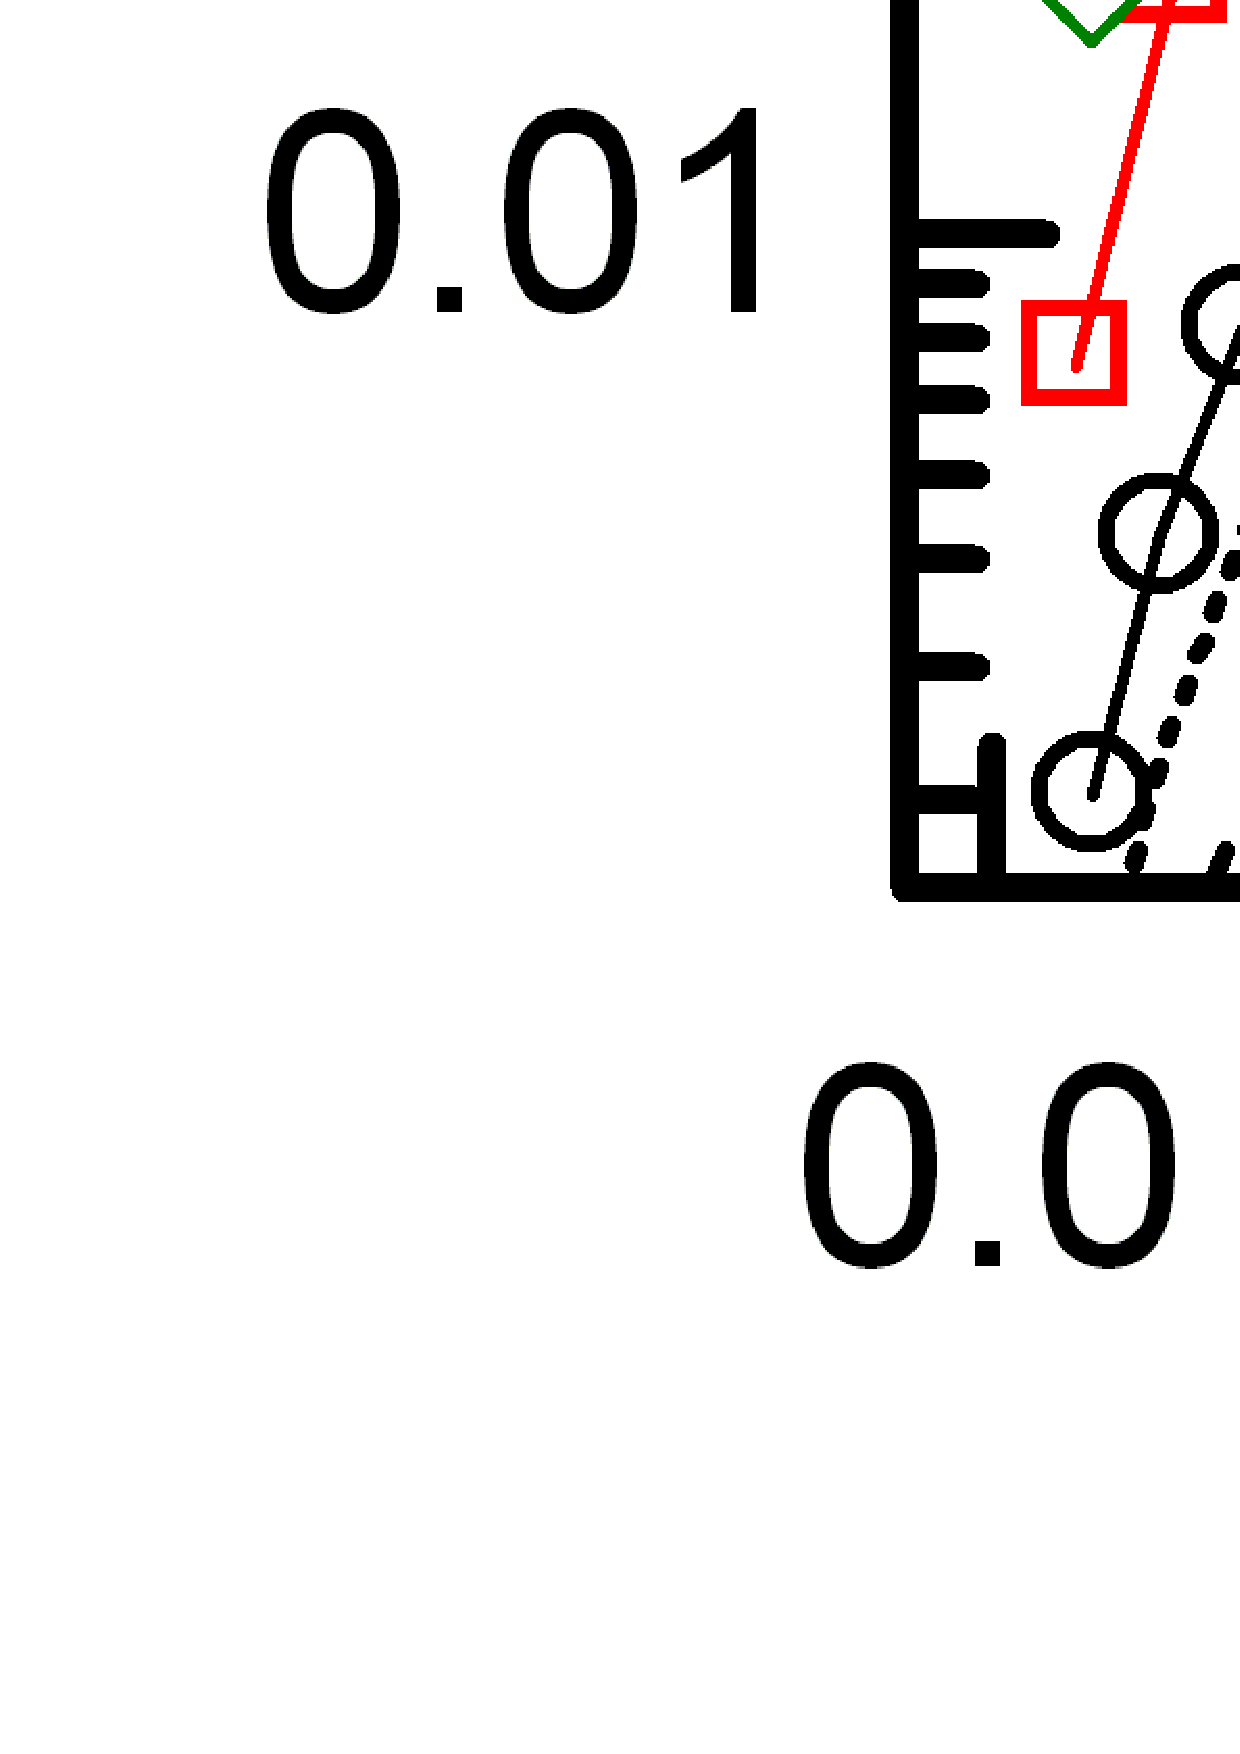
\includegraphics[width=0.9\textwidth]{olikhFig1}%
\caption{\label{figIV}
Dark $I$--$V$ characteristics measured (a) at 306~K for non--irradiated (circles), neutron--irradiated (squares) and gamma--irradiated (diamonds and triangles) structures without USL;
(b) at 301~K (circles) and 341~K (asterisks) with (filled marks, $W_{U\!S}=0.40$~W/cm$^2$) and without(open marks) USL for the iSC.
The marks are the experimental results, the solid lines are the fitted curves using Eqs.~(\ref{eqIV})--(\ref{eqW}).
The dashed, dot--dashed and dotted lines in (a) are the base, SCR and shunt components of iSC current, respectively.
}%
\end{figure*}

The double--diode model of n$^+$--p structure $I$--$V$ characteristics expressed in the following form:
\begin{eqnarray}
I(V,T)&=&I_{SCR}+I_{base}+I_{sh}\;,\label{eqIV}\\
I_{SCR}&=&\frac{qAn_id}{2\tau_{g}}\left\{\exp \left[\frac{q(V-IR_s)}{nkT}\right]-1\right\}\,,\label{eqIscr}\\
I_{base}&=&\frac{qAn_i^2}{p_p}\sqrt{\frac{\mu_nkT}{\tau_n}}\left\{\exp \left[\frac{q(V-IR_s)}{kT}\right]-1\right\},\label{eqIbase}\\
I_{sh}&=&(V-IR_s)/R_{sh}\,,\label{eqIsh}
\end{eqnarray}
where
$I_{SCR}$ reflects the overall recombination in the space charge region (SCR),
$I_{base}$ is closely related to recombination in the quasi-neutral region,
$I_{sh}$ is the shunt current,
$A$ is the sample area,
$n_i$ is the intrinsic carrier concentration,
$\tau_{g}$ is the SCR carrier lifetime,
$d$ is the  SCR thickness:
\begin{equation}
\label{eqW}
    d=\sqrt{\frac{2 \varepsilon \varepsilon_0(p_p+n_n)}{q^2 p_p n_n}\left[E_g-kT\ln\!\left(\frac{N_vN_c}{p_pn_n}\right)-2kT\!-\!Vq\right]},
\end{equation}
$\varepsilon$ is the permittivity (11.7 for Si),
$p_p$ and $n_n$ are the majority carrier concentration in the $p$-- and $n$--type regions,
$E_g$ is the semiconductor band gap,
$N_c$ and $N_v$ are the effective density of states in the conduction and valence bands;
$n$ is the ideality factor of the nonideal current components,
$R_s$ and $R_{sh}$ are the series and shunt resistances of the structure,
$\mu_n$ and $\tau_n$ are the electron (minority carrier) mobility and lifetime in the diode base.


We used Eqs. (\ref{eqIV})--(\ref{eqW}) to fit the experimental data and $\tau_g$, $\tau_n$, $n$, $R_{sh}$, and $R_s$ were taken as the  fittings parameters.
The known \cite{ni:Green,Schroder2006,Markvart} temperature dependencies of $n_i$, $E_g$, and $\mu_n$ were used.
The extremely good fit to the experimental data was obtained --- see Fig.~\ref{figIV}.
In particular, the $R_s$ value 1~$\Omega$ was determined for all samples.


In the USL case, the transverse acoustic waves with frequency of $4.2$~MHz were exited with help of a piezoelectric transducer and were injected in the samples from the base side in the [111]-direction.
The USLs parameters of different samples are listed in the Table~\ref{tabUSL}.
It was reported previously \cite{Ostapenko1995,Olikh:Ultras,Ostrovskii2001} that a characteristic time of change in the silicon structure parameters under the ultrasound action  did not exceed $2\cdot10^3$~s.
In order to wait till the acoustically induced (AI) transitional period the following experimental procedure has been used.
After USL start the sample was kept at room temperature during 60 min and then the $I$--$V$ measurements and the sample heating were started.
In order to avoid the effect of piezoelectric field on $I$--$V$ characteristics, the piezoelectric transducer has been shielded.


\begin{table}
\caption{\label{tabUSL}The parameters of ultrasound loadings.
}
\begin{ruledtabular}
\begin{tabular}{lcr}
Sample&$W_{U\!S}$, W/cm$^2$&Label\\
\hline
\multirow{2}{*}{iSC}&0.22&USL--i--1\\
&0.40&USL--i--2\\
\multirow{2}{*}{nSC}&0.21&USL--n--1\\
&0.36&USL--n--2\\
g6SC&0.32&USL--g6--2\\
\multirow{2}{*}{g7SC}&0.24&USL--g7--1\\
&0.40&USL--g7--2\\
\end{tabular}
\end{ruledtabular}
\end{table}


The linear and non-linear fitting were done by using the least-squares and differential evolution \cite{DEWang} method, respectively.


\section{Results and Discussion}
\subsection{Ultrasound influence on the SCR recombination
\label{P1}}



\section{Conclusion}
In this work, 16 methods were implemented to extract the physical parameters of Schottky diodes.
To do so, experimental and synthetic $I$--$V$ data were used.
It has been analyzed the dependences of extraction accuracy of series resistance, barrier height and ideality factor on the parameters value and on the noise level of the $I$--$V$ curve.
It has been shown that the use of Lambert function for numerical calculation allows to reduce both the determination error value and the number of accuracy influencing factor; whereas the running time increases.
It has been examined the adaptive procedure, which provide selection of the $I$--$V$ data range for an auxiliary function construction taking into account the deviation of calculated curve and curve under investigation.
This procedure find out to improve the accuracy of analytical Gromov method, especially in the case of low noise level data.
In consideration of evolutionary algorithms, the MABC method is favorable over the DE, the PSO and the TLBO due to the minimal running time.
The most reliable and preferred methods seem to be evolutionary algorithms (specifically the MABC), Gromov method with adaptive procedure and Lee method.
The first one is reasonable in the case of
a small $R_s$ value (a few ohms) or a large $I_s$ value (high temperature).

This work of review, test and comparative analysis of different techniques for determination of Schottky diode parameters should be useful for further research and development on metal-semiconductor devices.

\bibliography{olikh}



\end{document}

